\chapter{On-going studies}%
\label{sec:other_ana}


This section brings other studies that are on-going activities. Namely, they are
extrapolation to higher kinematic regime
(Section~\ref{ssec:kinematic_extrapolation}) and the \rnn{} employment for
boosted topologies (Section~\ref{ssec:boosted_topology}).

\section{Model Extrapolation to Higher Kinematic Regime}%
\label{ssec:kinematic_extrapolation}

% TODO Changes in pile-up correction for low-et

Most of the \Zee{} \tnp{} data is comprised within the $\et{}<\SI{100}{\GeV}$
region, whereas the single electron triggers become independent from
selection algorithms only when $\et{}>\SI{300}{\GeV}$. Hence, any electron trigger
development needs to consider the selection model extrapolation for the region
$100<\et{} [\text{\GeV}]<300$. It is particularly important given that electrons
have specific changes in the shower development around this
region~\cite{atlas_electron_id_offline}, i.e.\@ the increase in \emiii{} energy
leakage. There are two primary triggers covering the specific regions requiring
the \medium{} working point for $\et{}<\SI{140}{\GeV}$ and \vloose{} otherwise.
Hence, it suffices that a \medium{} trigger does not show lower efficiency in
the kinematic region to ensure that the selection model is able to extrapolate
well. Figure~\ref{fig:high_et_eff} shows the efficiency of a \medium{} electron
trigger using an early \rnn{} tune performed during the development stage with
respect to a trigger without \rnn{}. Despite the low statistics available, the
efficiency of both triggers match to the few per mile level in the high
kinematic region.




\begin{figure}[htb]
  \centering
  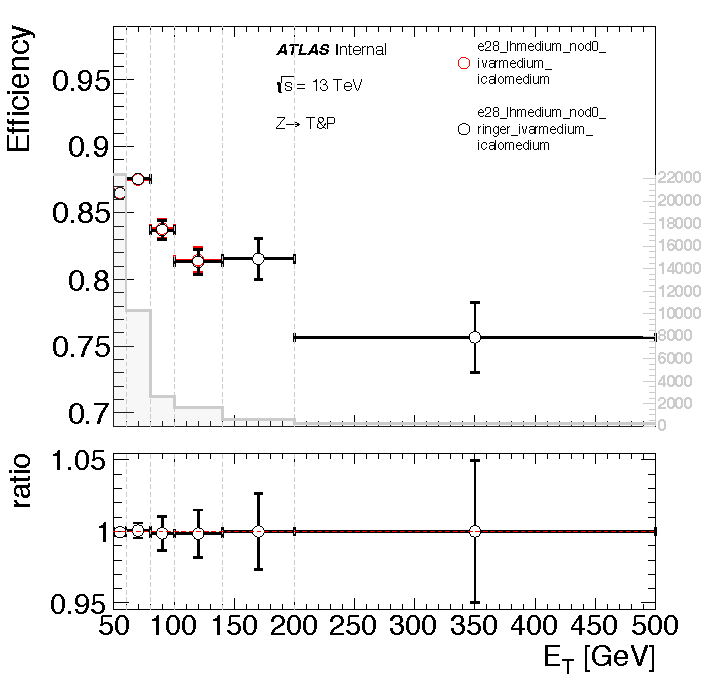
\includegraphics[width=.5\textwidth]{sections/other_studies/figures/high_et_e28_lhmedium_nod0}
  \caption{\Zee{} \tnp{} efficiency as a function of \et{} for triggering with
  \rnn{} in red and without it in black, both applying \medium{} selection
on ATR-16156 data reprocessing. On the right y-axis, the \tnp{} pair counts,
shown in the gray histogram. The bottom pad shows the efficiency ratio with
error bars computed assuming both triggers to be
uncorrelated.\label{fig:high_et_eff}}
% (error bars overestimated)
\end{figure}





We are evaluating the \rnn{} with simulations covering a larger kinematic region
($Z^{'}\rightarrow ee$ and Drell-Yan) processes and using additional triggers.

\section{Boosted Physics Configurations}\label{ssec:boosted_topology}



During Run~2, the \rnn{} algorithm employed a $0.2\times0.2$ window in the
\etaphi axis around the hottest cell. The window size goes beyond the standard
shower shapes coverage in order to capture additional discriminative
information. The training procedure considered only isolated electrons as signal
samples and the input patterns are normalized by the total energy. It is not
unexpected that, when another electron lies within the \rnn{} feature extraction
window, that the physics objects are discarded as shown in
Figure~\ref{fig:boosted_eff_dr}. These events will generate high activity in the
outer rings and depending on how strong it is with respect to the central
electron activity (due to the normalization), it will be beyond the expected
pile-up activity and hence display a profile similar to those available in jets.
Note that $\Delta$R results in a circular area whereas the \rnn{} feature
extraction is rectangular. Although both regions have a large overlap, there is
some discrepancy, which may be causing a smoother drop in efficiency around
$\Delta\text{R}=0.2$ in Figure~\ref{fig:boosted_eff_dr}. Other factors influencing the efficiency of the boosted system are
how balanced is the energy of both electrons and how much energy of
the non-central electron lies within
the window. We expect the worst case scenario to be when the outer electron has
nearly the same or higher energy than the central one.



\begin{figure}[h!tb]
\centering
\begin{subfigure}[c]{.48\textwidth}
\centering
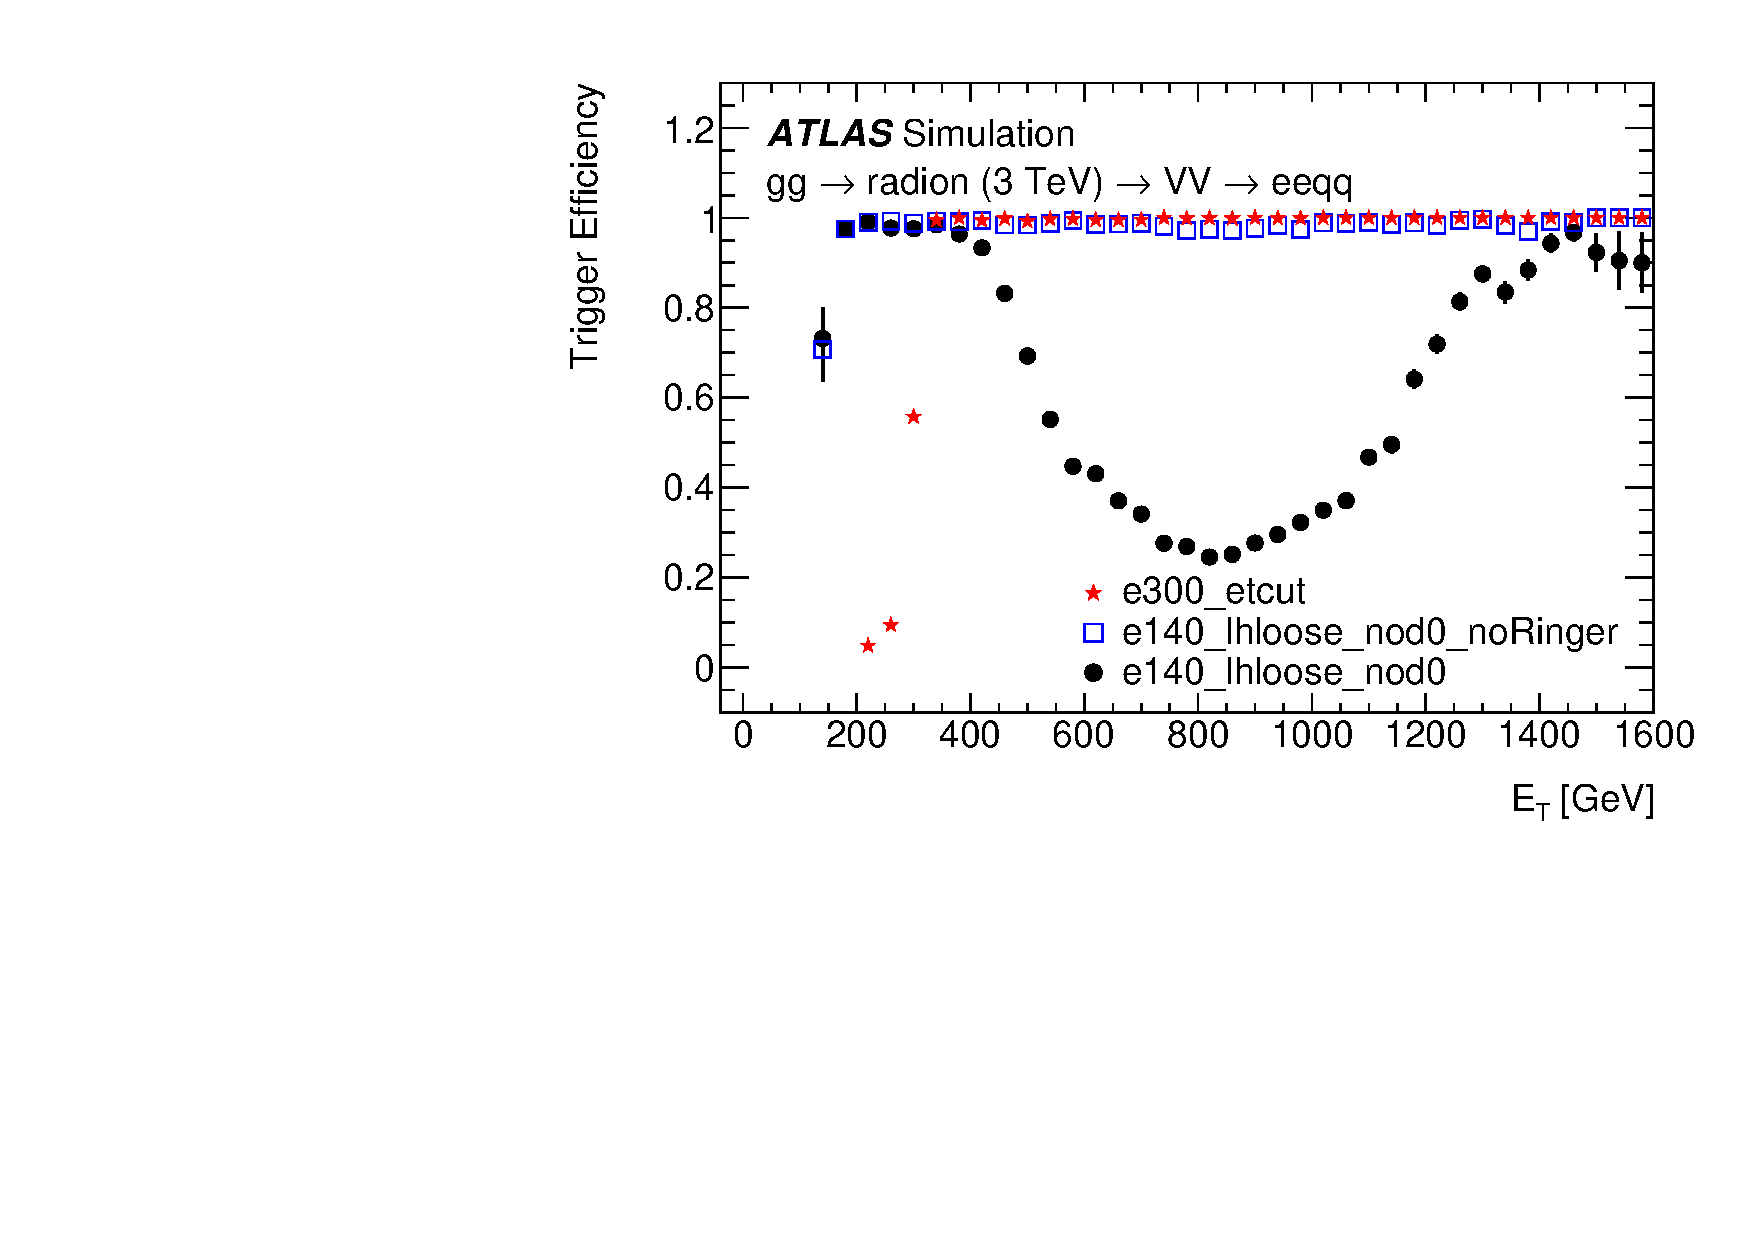
\includegraphics[width=\textwidth]{sections/other_studies/figures/public_plots/fig_13a}
\caption{}%
\label{fig:boosted_eff_et}
\end{subfigure}
\hfill
\begin{subfigure}[c]{.48\textwidth}
\centering
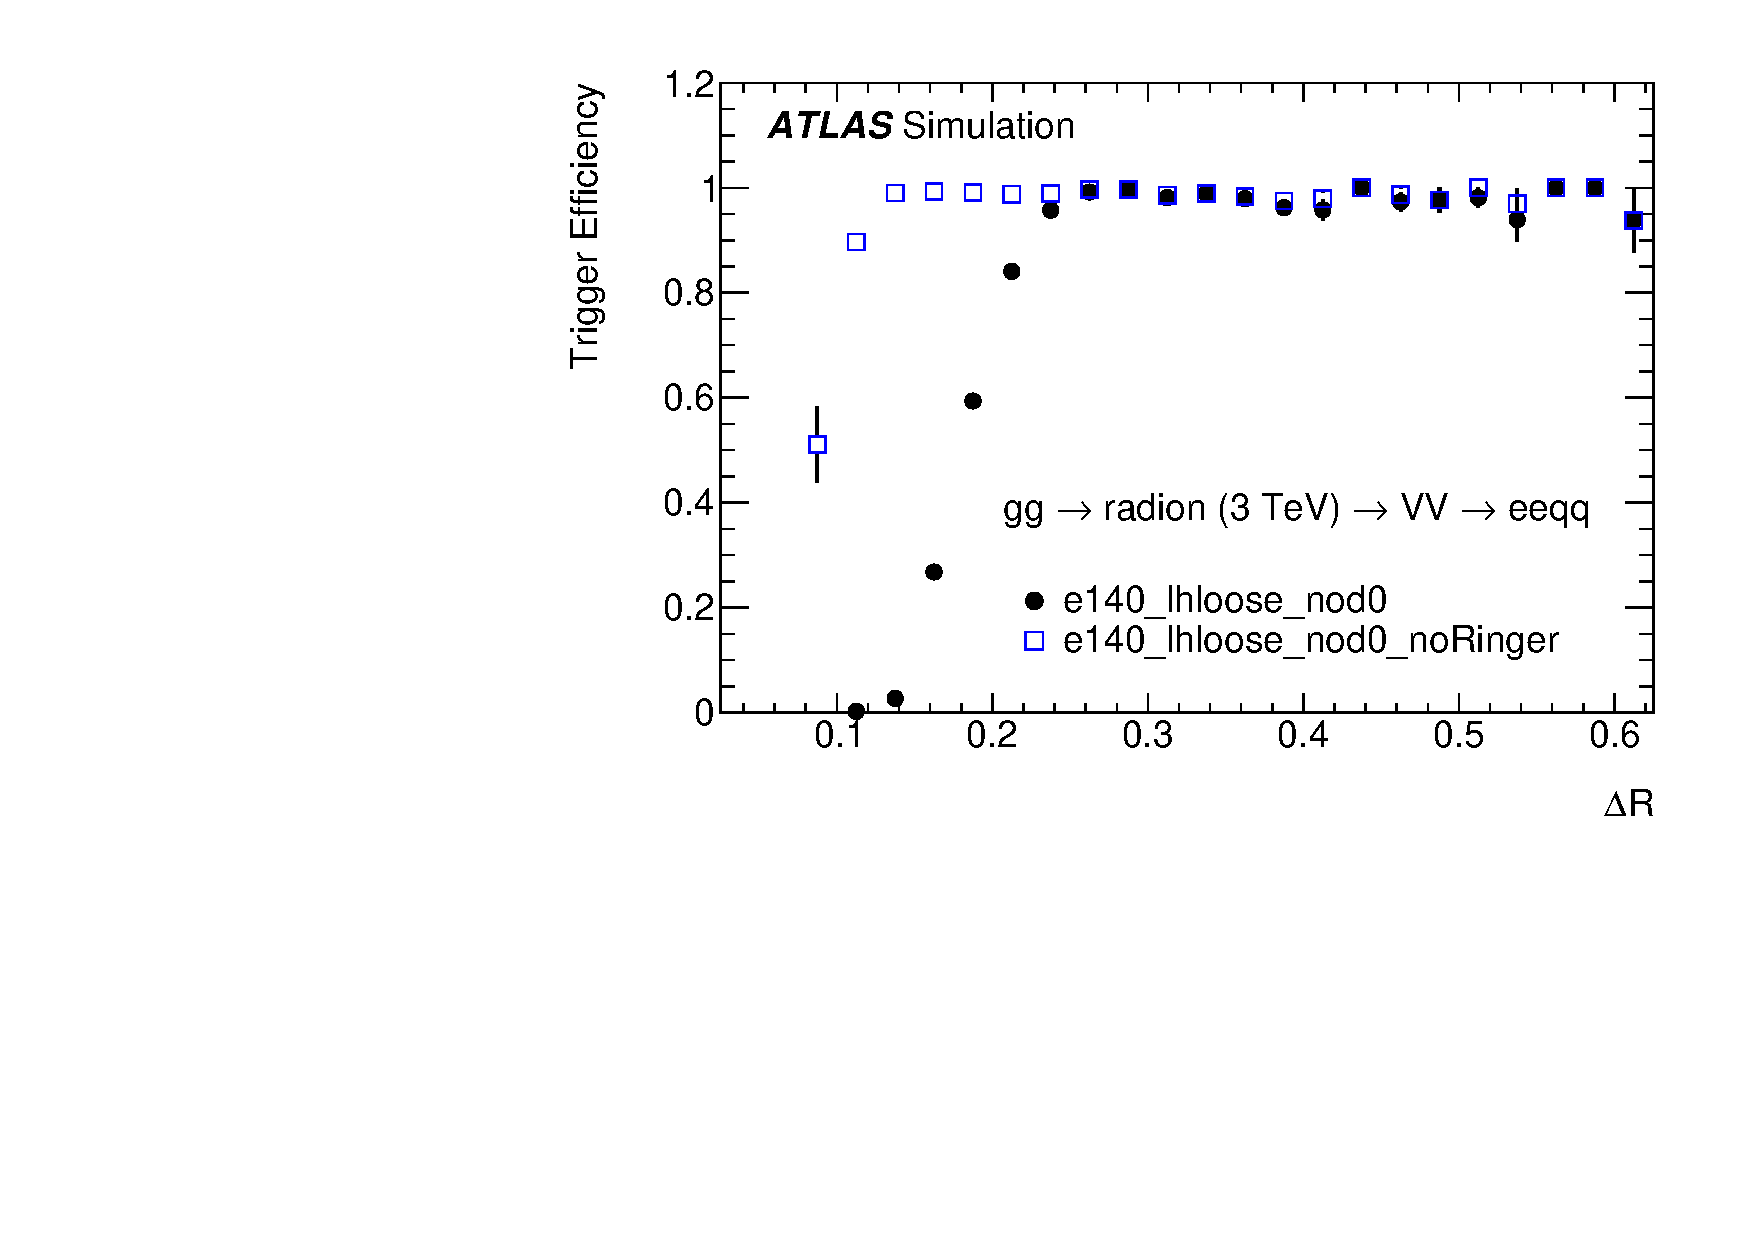
\includegraphics[width=\textwidth]{sections/other_studies/figures/public_plots/fig_13b}
\caption{}%
\label{fig:boosted_eff_dr}
\end{subfigure} \\
\caption{
The efficiency for electrons from gg $\rightarrow$ radion (3 TeV)
$\rightarrow$ VV $\rightarrow$ eeqq as a function of (a) the offline electron ET
and (b) $\Delta$R between two electrons. Efficiency is given with respect to
offline loose identification and the FCLoose isolation working point. For (b),
only offline candidates with $\et{} > \SI{400}{\GeV}$ are used to account only
for the range which can result in boosted configurations~\cite{aad2020performance}.
}%
\end{figure}





% TODO Ref for the radion

Figure~\ref{fig:boosted_eff_et} shows that the particular boosted topology,
consisting of merged electrons originating from radions, starts to result in
electrons within the feature extraction window when their transverse energies
are around \SI{400}{\GeV}. The triggering with \rnn{} recovers efficiency around
\SI{1.4}{\TeV} where either the two electrons become too near to each other or
the energy of the non-central electron becomes very small with respect to the
central one. For boosted topologies with electrons above \SI{300}{\GeV}, a
trigger is available regardless of the trigger selection strategy. Backup
triggers without the \rnn{} are also available covering lower kinematic regions.

We are currently developing a \rnn{}-based method to cover boosted
configurations while maintaining electron efficiency high.


